\subsection{Упражнение 1}

При взятии выборок из сигнала при слишком низкой чистоте кадров составляющие, большие частоты заворота дадут биения. В таком случаее эти компоненты не отфильтруешь, посколько они неотличимы от более низких частот. Полезно отфильтровать эти частоты до выборки: фильтр НЧ, используемый для этой цели, называется фильтром сглаживания. Вернитесь к примеру "Соло на барабане", примените фильтр НЧ до выборки, а затем, опять с помощью фильтра НЧ, удалите спектральные копии, вызванные выборкой. Результат должен быть идентицент отфильтрованному сигналу.

Возьмем звук барабанов, применим фильтр НЧ до выборки, а затем, опять с помощью фильтра НЧ удалим спектральные копии, вызванные выборкой.

\begin{lstlisting}[language=Python]
wave = read_wave('263868__kevcio__amen-break-a-160-bpm.wav')
wave.plot()
\end{lstlisting}
\begin{figure}[H]
	\begin{center}
		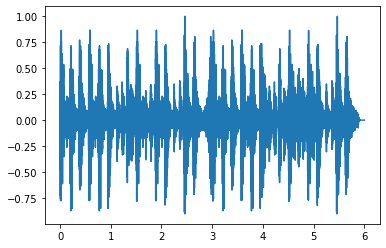
\includegraphics[scale=1]{fig/lab11/lab11_1.png}
		\caption{График звука барабанов}
	\end{center}
\end{figure}

\begin{lstlisting}[language=Python]
spectrum = wave.make_spectrum(full=True)
spectrum.plot()
\end{lstlisting}
\begin{figure}[H]
	\begin{center}
		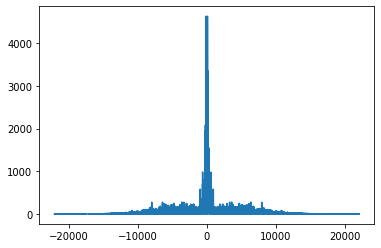
\includegraphics[scale=1]{fig/lab11/lab11_2.png}
		\caption{Спектр сигнала}
	\end{center}
\end{figure}

Применим фильтр низких частот:

\begin{lstlisting}[language=Python]
factor = 3
framerate = wave.framerate / factor
cutoff = framerate / 2 - 1

spectrum.low_pass(cutoff)
spectrum.plot()
\end{lstlisting}
\begin{figure}[H]
	\begin{center}
		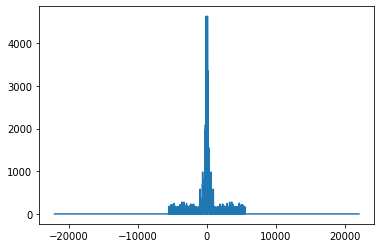
\includegraphics[scale=1]{fig/lab11/lab11_3.png}
		\caption{Отфильтрованный сигнал}
	\end{center}
\end{figure}

Применим функцию из учебника, которая имитирует процесс выборки.


\begin{lstlisting}[language=Python]
sampled = sample(filtered, factor)
sampled.make_audio()

sampled_spectrum = sampled.make_spectrum(full=True)
sampled_spectrum.plot()
\end{lstlisting}
\begin{figure}[H]
	\begin{center}
		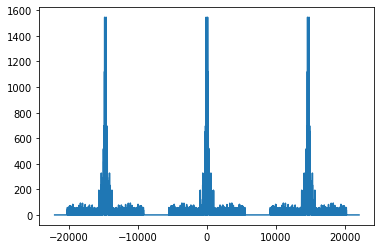
\includegraphics[scale=1]{fig/lab11/lab11_4.png}
		\caption{Получившийся спектр}
	\end{center}
\end{figure}


Теперь удалим спектральные копии:
\begin{lstlisting}[language=Python]
sampled_spectrum.low_pass(cutoff)
sampled_spectrum.plot()
\end{lstlisting}
\begin{figure}[H]
	\begin{center}
		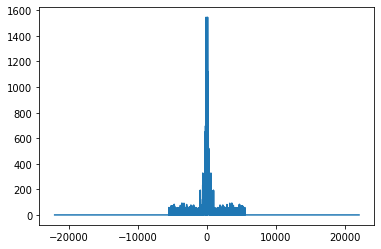
\includegraphics[scale=1]{fig/lab11/lab11_5.png}
		\caption{Результат избавления от копий}
	\end{center}
\end{figure}

Сравним звуки

\begin{lstlisting}[language=Python]
spectrum.make_wave().make_audio()

interpolated = sampled_spectrum.make_wave()
interpolated.make_audio()

spectrum.plot()
sampled_spectrum.plot()
\end{lstlisting}

\begin{figure}[H]
	\begin{center}
		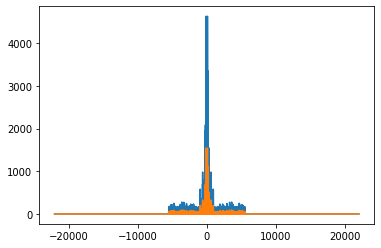
\includegraphics[scale=1]{fig/lab11/lab11_6.png}
		\caption{Сравнение спектров}
	\end{center}
\end{figure}

Звуки отличаются , увеличим амлитуду в три раза:

\begin{lstlisting}[language=Python]
sampled_spectrum.scale(factor)
sampled_spectrum.plot()
spectrum.plot()
\end{lstlisting}
\begin{figure}[H]
	\begin{center}
		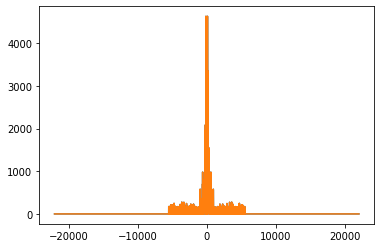
\includegraphics[scale=1]{fig/lab11/lab11_7.png}
		\caption{Сравнение спектров}
	\end{center}
\end{figure}

В итоге разница между интерполированной волной и фильтрованной волной есть, но она едва заметная.

\subsection{Вывод}

В данной работе были проверены свойства выборок и прояснены биения и заворот частот.
